% !TeX spellcheck = en_US
\chapter{Exploration}

\section{Overview}
In the setting of delayed reward, not knowing which actions would give more reward, we would want the agent to \textit{explore}. The concerns are:
\begin{itemize}
	\item How can an agent discover high-reward strategies that require a temporally extended sequence of complex behaviors that, individually, are not rewarding?
	\item How can an agent decide whether to attempt new behaviors (to discover ones with higher reward) or continue to do the best things it knows so far?
\end{itemize}
This poses a exploration and exploitation dilemma:
\begin{itemize}
	\item \textit{Exploration}: doing things you haven't done before, in the hopes of getting even higher reward
	\item \textit{Exploitation}: doing what you know will yield the highest reward
\end{itemize}

\subsection{Regret}
\label{sec:regret}
Exploration can be viewed as a \ac{POMDP}. Solving the \ac{POMDP} to know the exact underlying distribution is overkill. We instead want a simpler strategy that is not too bad from the optimal ones. The \textit{regret} is the metric to measure how good or bad an exploration strategy.

\hlb{Definition:} \textit{Regret} is the reward difference from optimal policy at time step $T$:
\begin{align*}
	&\underbrace{Reg(T)}_{\textstyle \text{regret at $T$}} = &&T. \underbrace{\mathbb{E}[r(a^*)]}_{\textstyle \text{expected reward of the best action}} && - \underbrace{\sum_{t=1}^T r(a_t)}_{\textstyle \text{the actual sum of reward}}
\end{align*}

\hlb{Example:} Consider the following multi-armed bandit problem:\\
A professor moves to a small town for work. He will stay there for 300 days. Each day, he will eat at one of three restaurants in the town. Eating at each restaurant has a different happiness distribution. Let say, the happiness distributions of each restaurant are as follows:
\begin{itemize}
	\item Restaurant 1: $\mu=10, \sigma=5$
	\item Restaurant 2: $\mu=8, \sigma=8$
	\item Restaurant 3: $\mu=5, \sigma=25$
\end{itemize}
\textbf{Not knowing the true happiness distribution, which strategy should the professor follow to maximize the expected happiness score?}

The regrets for some exploration strategies:
\begin{itemize}
	\item Optimal reward: Knowing the true distribution, the optimal action is to always go to restaurant 1.
	\[ \mathbb{E}[r] = 300 \times 10 = 3000\]
	\item Explore only: the professor spends 100 days at each restaurant.
	\begin{align*}
		\mathbb{E}[r] &= 100 \times 10 + 100 \times 8 + 100 \times 5 = 2300\\
		\Rightarrow \rho &= 3000 - 2300 = 700 \qquad \text{(regret)}
	\end{align*}
	\item Exploit only: visit each restaurant once, then stick with the one with the highest value.\\
	Assume the receive reward after 3 days are: $r_1 = 7, r_2 = 8, r_3 = 5$. After that, the expected reward would be:
	\[ \mathbb{E}[r] = 7 + 8 + 5 + (300 - 3) \times 8 = 2396 \]
	However, this is not the actual expected reward for the exploit only strategy.
	\[\rho = 3000 - 2670 = 330\]
	\item Zero regret strategy: As time goes on $T\rightarrow \infty$, the regret will approach to 0 $\rho \rightarrow0$
\end{itemize}

\subsection{Optimality}
\textit{Optimality}: An exploration strategy is \textit{optimal} when we compared the regret \ac{vs} the Bayes-optimal strategy. \todo{}

\todo{Optimal exploration in small \ac{MDP}s}

\subsection{Tractability}
\begin{itemize}
	\item With \textit{theoretically tractable} exploration strategy, we can quantify or understand whether the given exploration strategy is optimal or sub-optimal
	\item With \textit{theoretically intractable} exploration strategy, we cannot make the above estimate exactly.
\end{itemize}

\begin{center}
	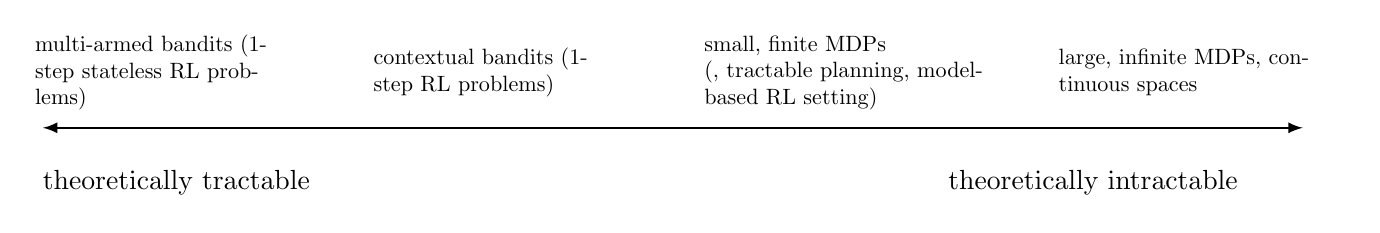
\begin{tikzpicture}
		\draw[thick,latex-latex] (-8,0) -- (8,0);
		\node[text width=5cm] at (-5.5,-.7) {theoretically tractable};
		\node[text width=5cm] at (6,-.7) {theoretically intractable};			
		\node[scale=0.8, text width=4cm] at (-6.5,.7) {multi-armed bandits (1-step stateless \ac{RL} problems)};
		\node[scale=0.8, text width=4cm] at (-2.2,.7) {contextual bandits (1-step \ac{RL} problems)};
		\node[scale=0.8, text width=4.5cm] at (2.2,.7) {small, finite \ac{MDP}s\newline (\eg, tractable planning, model-based \ac{RL} setting)};
		\node[scale=0.8, text width=4cm] at (6.5,.7) {large, infinite \ac{MDP}s, continuous spaces};
	\end{tikzpicture}
\end{center}

\begin{itemize}
	\item multi-armed bandits: can formalize exploration as \ac{POMDP} identification
	\item contextual bandits: policy learning is trivial even with \ac{POMDP}
	\item small, finite \ac{MDP}s: can frame as Bayesian model identification, reason explicitly about value of information
	\item large or infinite \ac{MDP}s: optimal methods don’t work, but can take inspiration from optimal methods in smaller settings
\end{itemize}

\section{Bandits Problems}
\subsection{One-Armed Bandit}
One armed bandit is the slot machine. It can be represent as a \ac{MDP} with one single action. The \ac{prob} distribution of the reward is unknown.
\begin{align}
	&\mathcal{A} = \{\text{pull arm}\}\\
	&r(\text{pull arm}) = ?
\end{align}

\begin{figure}[hbt!]
	\centering
	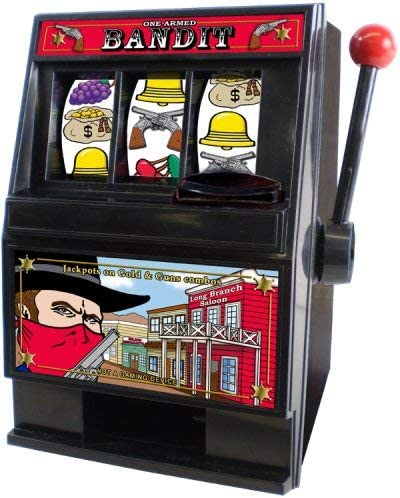
\includegraphics[width=.2\textwidth]{one-armed-bandit.png}
	\caption{One-armed bandit (\href{https://www.amazon.com/Armed-Bandit-Slot-Machine-Bank/dp/B001KYV9DW}{src}).}
\end{figure}

\subsection{Multi-Armed Bandit}
Multi armed bandit is a bank of multiple one-armed bandit slot machines. This problem is a 1-step stateless \ac{MDP}. Different machines have different reward distributions, which are unknown, but can be learned by trials.
\begin{align}
	&\mathcal{A} = \{\text{pull}_1, \text{pull}_2, \dots, \text{pull}_n\}\\
	&r(a_n) = ?\\
	&\text{assume } r(a_n) \sim p(r|a_n)
\end{align}

We can define the bandits as a \ac{POMDP} with the state as \ac{param} that represents the reward models. Solving the \ac{POMDP} leads to the optimal exploration strategy.
\[ \textbf{s} = [\theta_1, \dots, \theta_n]\]
But the belief state of $\theta$ is large, thus, doing this is overkill. We can do well with simpler strategies.

\subsection{Contextual Bandits}
\begin{itemize}
	\item the reward distribution depends on some external measurable variable.
	\item bandits with state, essentially 1-step \ac{MDP}
	\item \todo{}
\end{itemize}

\subsection{Bandit Variants}
\begin{itemize}
	\item Infinite Arms: there are more slot machines.
	\item Variable Arms: the reward distribution varies for each slot machine.
	\item Combinatorial Bandits: the agent has to pull more than one arm at once.
	\item Dueling Bandits: agent always pulls two arms, is never told about the reward, \dots
	\item Continuous Bandits: agent has to choose interval value, like the force to the arm.
	\item Adversarial Arms: the agent plays against an opponent. Thus if the agent uses the same strategy, the opponent will adapt, and the Q-value of that action will change over time. \Eg: chess, tic-tac-toe.
	\item Strategic Arms
	\item and more!
\end{itemize}

\subsection{Gradient Bandits}
\todo{}

\subsection{Applications}
There are various applications in:
\begin{itemize}
	\item Ad serving: arms - possible ads, reward - a click
	\item Website optimization: arms: possible website options, reward - user engagement
	\item Clinical trials: arms: possible medications, reward - health outcomes
\end{itemize}

\section{Exploration Strategies for Bandits Problem}
\subsection{$\epsilon$-first}
\todo{}

\subsection{$\epsilon$-greedy}
\todo{formula}

With the example in \secref{sec:regret}, assuming $\epsilon = 10\%$, the professor spend 10\% of the days (30 days) to try non-optimal restaurants, and the rest to exploit the current belief about the best restaurant.
\[\rho \approx 100\]

\subsection{Optimistic Exploration}
\label{subsec:bandits-optimistic-exploration}
The high-level idea is to try each arm until you are sure it's not great.
\begin{itemize}
	\item Keep track of average reward $\widehat{\mu}_a$ for each action $a$
	\item Optimistic estimate: $a = \underset{a}{\arg\max} [\widehat{\mu}_a + C \sigma_a]$.\\
	Choose the action with either current high average reward, or with high covariance $\sigma_a$
\end{itemize}

\ac{UCB}:
\[ A_t = \underset{a}{\arg\max} \left[ Q_t(a) + c\sqrt{\frac{\ln t}{N_t(a)}}\; \right], \qquad\begin{cases}
	Q_t(a) - \text{current reward belief}\\
	N_t(a) - \text{\ac{no} times taking action $a$}\\
	t - \text{current \ac{no} time step}
\end{cases} \]

\ac{UCB}-1 use Chernoff - Hoeffding Inequality, with $Reg(T) = \mathcal{O}(\log T)$:
\[ C_j(t) = \sqrt{\frac{\log(n)}{T_j(t	)}} \]
\[ a = \underset{a}{\arg\max} \left[\widehat{\mu}_a + \sqrt{\frac{2\ln T}{N(a)}}\;\right] \]
\note
\begin{itemize}
	\item lots of other functions work as well, as long as they decrease with $N(a)$
	\item \ac{UCB} is more difficult than $\epsilon$-greedy to extend beyond bandits to more general \ac{RL} problems (nonstationary problems, large state spaces)
\end{itemize}

\subsection{Probability Matching / Posterior Sampling}
\label{subsec:bandits-posterior-sampling}
Optimistic strategy doesn't try to model the uncertainty. It is model-free approach, simply keeps the average rewards and the number of times an action is taken. For the multi bandits problem, assuming some reward model $r(a_i)\sim p_{\theta_i}(r_i)$, we could instead keep a belief $\widehat{p}(\theta_1, \dots, \theta_n)$ over the \ac{param} and solve the \ac{POMDP} with $\textbf{s} = [\theta_1, \dots, \theta_n]$.

\hlb{Idea:} Thompson sampling \cite{chapelle2011empirical}
\begin{enumerate}
	\item \tikzmark{pm1}Sample $\theta_1, \dots, \theta_n \sim \widehat{p}(\theta_1, \dots, \theta_n)$
	\item Pretend the model $\theta_1, \dots, \theta_n$ is correct
	\item Take the optimal action $a = \underset{a}{\arg\max} \mathbb{E}_{\theta_a} [r(a)]$
	\item \tikzmark{pm4}Update the model
	\begin{tikzpicture}[overlay,remember picture]
		\draw[very thick, -latex]
		([xshift=-7mm,yshift=1mm]pic cs:pm4) --++ (-.5,0) |-
		([xshift=-7mm,yshift=1mm]pic cs:pm1);
	\end{tikzpicture}
\end{enumerate}

\begin{itemize}
	\item Harder to analyze theoretically
	\item Can work very well empirically
\end{itemize}

\subsection{Information Gain}
\label{subsec:bandits-information-gain}
This method is even more explicitly model-based.

\hlb{Bayesian experimental design:} aim to determine some unknown latent variable $z$ but can only take actions to learn about it.
\begin{align*}
	&\mathcal{H}(\widehat{p}(z)) &&-\text{the current entropy of $z$ estimate}\\
	&\mathcal{H}(\widehat{p}(z)|y) &&-\text{the entropy of $z$ estimate after observation $y$}\\
	&IG(z,y) = \mathbb{E}_y \big[\mathcal{H}(\widehat{p}(z)) - \mathcal{H}(\widehat{p}(z)|y)\big] &&-\text{the \textit{information gain} about $z$ after $y$}\\
	&IG(z,y | a) = \mathbb{E}_y \big[\mathcal{H}(\widehat{p}(z)) - \mathcal{H}(\widehat{p}(z)|y) | a\big] &&-\text{usually condition on action $a$}
\end{align*}

\begin{itemize}
	\item \eg, $y$ might be optimal action $a^*$ or the reward $r(a)$)
	\item We want to take actions and receive $y$ such that we get high \ac{IG} about $z$
\end{itemize}

\Eg, bandit \ac{algor} \cite{russo2014learning}:
\begin{align}
	& y = r_a && -\text{reward for action $a$}\\
	& z = \theta_a && -\text{\ac{param} of model $p(r_a)$} \\
	& g(a) = IG(\theta_a, r_a | a) && -\text{information gain of } a\\
	& \Delta(a) = \mathbb{E}[ r(a^*) - r(a) ] && -\text{expected suboptimality of } a\\
	\Rightarrow & a = \underset{a}{\arg\min} \frac{\Delta(a)^2}{g(a)}
\end{align}
the high-level idea is to take the least suboptimal action that give us more information.

\todo{Bayesian Model-based \ac{RL}}\\
\todo{\ac{PAC} exploration}

\section{Exploration Strategies in RL}
\subsection{Information Theoretic Quantities in RL}
\begin{align*}
	&\pi(\textbf{s}) = p_\pi(\textbf{s}) &&-\text{state \textit{marginal} distribution of policy $\pi$}\\
	&\mathcal{H}(\pi(\textbf{s})) &&-\text{state \textit{marginal} entropy of policy $\pi$}\\
	&\mathcal{I}(\textbf{x;y}) = D_{KL} \big( p(\textbf{x,y}) || p(\textbf{x}) p(\textbf{y}) \big) &&-\text{mutual information (\href{math_notes.pdf}{math notes})}\\
	&\mathcal{I}(\textbf{s}_{t+1};\textbf{a}_t) = \mathcal{H}(\textbf{s}_{t+1}) - \mathcal{H}(\textbf{s}_{t+1} | \textbf{a}_t) &&-\text{\textit{empowerment}}	
\end{align*}

\hlb{Intuition:} we want a large empowerment because: A large entropy $\mathcal{H} (\textbf{s}_{t+1})$ implies that there are many possible next states. A small entropy $\mathcal{H}(\textbf{s}_{t+1} | \textbf{a}_t)$ implies that given current action, it's easy to determine where the state will landed.

\subsection{Optimistic Exploration in Deep RL}
For bandits problem, \ac{UCB} chooses the action with $a = \underset{a}{\arg\max} \widehat{\mu}_a + \sqrt{\frac{2\ln T}{N(a)}}$ (\subsecref{subsec:bandits-optimistic-exploration}). The term $\sqrt{\frac{2\ln T}{N(a)}}$ can be considered as "exploration bonus". Lots of functions work, as long as they decrease with the count $N(a)$.

For \ac{MDP}s, we use similar state counts $N(\textbf{s, a})$ or $N(\textbf{s})$ to add \textit{exploration bonus}:
\begin{align}
	&r^+(\textbf{s,a}) = r(\textbf{s,a}) + \mathcal{B}(N(s)) && -\text{updated reward function}\\
	&\mathcal{B}(N(s)) && -\text{bonus that decreases with $N(\textbf{s})$}
\end{align}
\[\begin{matrix*}[l]
	\color{Green}+ \text{simple addition to any model-free \ac{RL} \ac{algor}}\\
	\color{red}- \text{need to tune bonus weight}
\end{matrix*}\]

In most settings of continuous state and action space, the agent might not literally visit the exact state again.\\
$\Rightarrow$ \hlb{Pseudo-counts:} to count similar states $\hat{N}(\textbf{s})$ or $\hat{N}(\textbf{s,a})$ \cite{bellemare2016unifying}
\begin{enumerate}
	\item \tikzmark{pc1}fit model $p_\theta(\textbf{s})$ to all states $\mathcal{D}$ seen so far
	\item take a step $i$ and observe $\textbf{s}_i$
	\item fit new model $p_{\theta'}(\textbf{s})$ to $\mathcal{D} \bigcup \textbf{s}_i$
	\item use $p_{\theta}(\textbf{s}_i)$ and $p_{\theta'}(\textbf{s}_i)$ to estimate $\hat{N}(\textbf{s})$
	\item \tikzmark{pc5}set $r_i^+ = r_i + \mathcal{B}(\hat{N}(\textbf{s}))$
	\begin{tikzpicture}[overlay,remember picture]
		\draw[very thick, -latex]
		([xshift=-7mm,yshift=1mm]pic cs:pc5) --++ (-.5,0) |-
		([xshift=-7mm,yshift=1mm]pic cs:pc1);
	\end{tikzpicture}
\end{enumerate}
\[ \hat{N}(\textbf{s}_i) = \hat{n} p_\theta(\textbf{s}_i), \qquad \hat{n} = \frac{1 - p_{\theta'}(\textbf{s}_i)}{p_{\theta'}(\textbf{s}_i) - p_\theta(\textbf{s}_i)} p_\theta(\textbf{s}_i) \]

\hlb{Types of exploration bonus:}
\begin{align}
	&- \text{\ac{UCB}:} &&\mathcal{B}(N(\textbf{s})) = \sqrt{\frac{2\ln n}{N(\textbf{s})}}\\
	&- \text{MBIE-EB: \cite{strehl2008analysis, bellemare2016unifying}} &&\mathcal{B}(N(\textbf{s})) = \sqrt{\frac{1}{N(\textbf{s})}}\\
	&- \text{BEB: \cite{kolter2009near}} &&\mathcal{B}(N(\textbf{s})) = \frac{1}{N(\textbf{s})}
\end{align}

\hlb{Kind of model:} $p_\theta(\textbf{s})$ need to output densities, but not necessarily produce great samples
\begin{itemize}
	\item CTS model \cite{bellemare2016unifying}
	\item stochastic neural networks
	\item compression length
	\item EX2
\end{itemize}

There are similar count style approaches:
\begin{itemize}
	\item Counting with hashes: counts states but in different space \cite{tang2017exploration}.
	\item Implicit density modeling with exemplar models: Use a classifier to classify whether a state is \textbf{novel} or not. \cite{fu2017ex2}
	\item Heuristics estimation of counts via errors: Given buffer $\mathcal{D} = \{(\textbf{s}_i, \textbf{a}_i)\}$
	\begin{itemize}
		\item Fit $\hat{f}_\theta(\textbf{s,a})$ to \textbf{target} function $f^*(\textbf{s,a})$
		\item Use $\mathcal{E}(\textbf{s,a}) = \left|\left| \hat{f}_\theta(\textbf{s,a}) - f^*(\textbf{s,a}) \right|\right|^2$ as exploration bonus
	\end{itemize}
	Choice for $f^*(\textbf{s,a})$: \cite{burda2018exploration}
	\begin{itemize}
		\item $f^*(\textbf{s,a}) = \textbf{s}'$ as next state transition
		\item $f^*(\textbf{s,a}) = f_\phi(\textbf{s,a})$, where $\phi$ is a \textit{random} \ac{param} vector
	\end{itemize}
	
\end{itemize}

\subsection{Posterior Sampling in Deep RL}
The \ac{MDP} analog for $\theta$ of the bandits problem (\subsecref{subsec:bandits-posterior-sampling}) is the Q-function.

\hlb{Idea:}
\begin{enumerate}
	\item \tikzmark{ts1}sample Q-function $Q$ from $p(Q)$
	\item act according to $Q$ for one episode
	\item \tikzmark{ts3}update $p(Q)$	
	\begin{tikzpicture}[overlay,remember picture]
		\draw[very thick, -latex]
		([xshift=-7mm,yshift=1mm]pic cs:ts3) --++ (-.5,0) |-
		([xshift=-7mm,yshift=1mm]pic cs:ts1);
	\end{tikzpicture}
\end{enumerate}

\hlb{Bootstrapped \ac{DQN} algorithm:} to represent the distribution of a function \cite{osband2016deep}
\begin{itemize}
	\item given a dataset $\mathcal{D}$, resample with replacement $N$ times $\rightarrow$ $\mathcal{D}_1, \dots, \mathcal{D}_N$
	\item train each model $f_{\theta_i}$ on $\mathcal{D}$ (\note shared network with multi heads)
	\item to sample from $p(Q)$, sample $i \in [1, \dots, N]$ and use model $f_{\theta_i}$
\end{itemize}
\[\begin{matrix*}[l]
	\color{Green}+ \text{no change to original reward function}\\
	\color{red}- \text{very good bonuses often do better}
\end{matrix*}\]

\subsection{Information Gain in Deep RL}
Extending \subsecref{subsec:bandits-information-gain} in the context of deep \ac{RL}:
\begin{itemize}
	\item \ac{IG} on reward $r(\textbf{s,a})$: not very useful if reward is sparse
	\item \ac{IG} on state density $p(\textbf{s})$: strange, but makes sense!
	\item \ac{IG} on dynamics $p(\textbf{s}'|\textbf{s,a})$: good proxy for learning \ac{MDP}, though still heuristics
	\item Generally intractable to use \ac{IG} exactly, thus, we will \hlb{have to approximate something}
\end{itemize}

Few options for approximation of \ac{IG} are:
\begin{itemize}
	\item Prediction gain: $\log p_{\theta'}(\textbf{s}) - \log p_{\theta}(\textbf{s})$ \cite{bellemare2016unifying}\\
	\hlb{Intuition:} if the density change a lot, the state was novel
	\item Variational inference: $D_{KL} \big( p(z|y) || p(z) \big)$\\
	Learn about \textit{transitions} $p_\theta (s_{t+1}|s_t, a_t)$, with $z=\theta$ and $y=(s_{t+1}|s_t, a_t)$
	\begin{align}
		\Rightarrow&D_{KL} \big( p(\theta|h, s_t, a_t, s_{t+1}) || p(\theta|h) \big) && -\text{\ac{IG} from a new transition}\\
		&h && -\text{history of all prior transitions}
	\end{align}
	\hlb{Intuition:} a transition is more informative if it causes belief over $\theta$ to change a lot.\\
	\hlb{Idea:} \cite{houthooft2016vime}
	\begin{itemize}
		\item Use variational inference to estimate $q(\theta|\phi) \approx p(\theta|h)$
		\item Given new transition $(s,a,s')$, update $\phi$ to get $\phi'$
		\item Use $D_{KL} \big( q(\theta|\phi') || q(\theta|\phi)\big)$ as approximate bonus of \ac{IG}
	\end{itemize}
\end{itemize}
\[\begin{matrix*}[l]
	\color{Green}+ \text{appealing mathematical formalism}\\
	\color{red}- \text{models are more complex, generally harder to use effectively}
\end{matrix*}\]

Similar works: exploration with model errors: \cite{schmidhuber2010formal, stadie2015incentivizing}

\section{Unsupervised Learning of Diverse Behaviors}
The three above approaches are modifications to existing \ac{RL} approaches to boost exploration behaviors, which is in the context of given existing task and reward. This section concerns situations there is no specified task, no sparse or delay reward, but \hlb{no reward at all}.
\begin{itemize}
	\item Learn skills without supervision, then use them to accomplish goals
	\item Learn sub-skills to use with hierarchical \ac{RL}
	\item Explore the space of possible behaviors
\end{itemize}

\subsection{Goal-proposed Mechanism}
\hlb{Intuition:} To prepare for an unknown goal in the future, the robot will have an unsupervised learning phase, in which it trains itself with self-proposed goals. The \textit{goal}, which is to reach an underlying state $z$, are inferred from current observation $x$, using variational inference models.

\hlb{Algorithm:} unsupervised goal-proposed mechanism
\begin{enumerate}
	\item \tikzmark{usl1}Propose goal: $z_g \sim p(z), x_g \sim p_\theta(x_g, z_g)$
	\item Attempt to reach goal using $\pi(a | x, x_g)$, reach $\bar{x}$
	\item Use data o update $\pi$
	\item \tikzmark{usl4}Use data to update $p_\theta(x_g | z_g), q_\phi(z_g | x_g)$
	\begin{tikzpicture}[overlay,remember picture]
		\draw[very thick, -latex]
		([xshift=-7mm,yshift=1mm]pic cs:usl4) --++ (-.5,0) |-
		([xshift=-7mm,yshift=1mm]pic cs:usl1);
	\end{tikzpicture}
\end{enumerate}

\hlb{How to have diverse goals?}\\
The initial policy $\pi$ might ends up with a specific state distribution $\pi(\textbf{s})=p_\pi(\textbf{s})$, which is not the marginal state distribution $p(\textbf{s}) \neq \pi(\textbf{s})$. If we use these samples to update the variational inference model, the model will learn and generate more samples similar to the seen samples. We don't want this to happen, thus, apply exploration ideas. \cite{nair2018visual, pong2019skew}
\begin{itemize}
	\item Standard \ac{MLE}: $\theta, \phi \leftarrow \underset{\theta, \phi}{\arg\max} \mathbb{E} [\log p(\bar{x})]$
	\item Weighted \ac{MLE}: $\theta, \phi \leftarrow \underset{\theta, \phi}{\arg\max} \mathbb{E} [w(\bar{x}) \log p(\bar{x})],\quad w(\bar{x}) = p_\theta (\bar{x})^\alpha,\quad \alpha\in \left[-1,0\right)$
\end{itemize}

\note the goal of unsupervised learning of diverse behaviors
\begin{itemize}
	\item Updating the variational inference model implies maximizing the entropy $\mathcal{H}(p(G))$ to have diverse goals
	\item Updating the policy $\pi(a|S,G)$ is minimizing $\mathcal{H}(p(G|S))$, because as $\pi$ gets better, the final state $S$ gets closer to $G$
	\item Thus, this algorithm is maximizing the empowerment $\max \mathcal{I}(S;G)$, good exploration $\mathcal{H}(p(G))$ and effective goal reaching $\mathcal{H}(p(G|S))$.
\end{itemize}


\subsection{State Distribution-Matching Formulation}
The first three types of \ac{algor}s, especially optimistic and \ac{IG}, have an intrinsic motivation to reward visiting \hlb{novel} states by adding an exploration bonus. This bonus concerns with whether the state has been visited \textit{often} before.
\begin{equation}
	\tilde{r}(\textbf{s}) = r(\textbf{s}) - \log p_\pi(\textbf{s}) = r(\textbf{s}) - \log\pi(\textbf{s})
	\label{eq:exploration-bonus}
\end{equation}

A general procedure could be described as:
\begin{enumerate}
	\item \tikzmark{sdm1} update $\pi(\textbf{a|s})$ to maximize $\mathbb{E}_\pi [\tilde{r}(\textbf{s})]$
	\item \tikzmark{sdm2} update $p_\pi(\textbf{s})$ to fit state marginal	
	\begin{tikzpicture}[overlay,remember picture]
		\draw[very thick, -latex]
		([xshift=-7mm,yshift=1mm]pic cs:sdm2) --++ (-.5,0) |-
		([xshift=-7mm,yshift=1mm]pic cs:sdm1);
	\end{tikzpicture}
\end{enumerate}

In the case of unsupervised learning with no reward $r(\textbf{s})$, the goal will then to simply to maximize the exploration bonus $ \tilde{r}(\textbf{s}) = - \log p_\pi(\textbf{s})$ (\eqref{eq:exploration-bonus}).

\hlb{Problem:} the state \ac{prob} is under expectation of the current policy $\pi$. Thus, the policy $\pi$ will keep changing to visit states that it hasn't been often before.

\hlb{Solution:} the state marginal matching problem - learn $\pi(\textbf{a|s})$ to minimize $D_{KL} \big( p_\pi(\textbf{s}) || p^*(\textbf{s}) \big)$
\begin{equation}
	\tilde{r}(\textbf{s}) = \log p^*(\textbf{s}) - \log p_\pi(\textbf{s})
\end{equation}

\begin{enumerate}
	\item \tikzmark{smm1}learn $\pi_k (\textbf{a|s})$ to maximize $\mathbb{E}_\pi [\tilde{r}(\textbf{s})]$
	\item \tikzmark{smm2}update $p_{\pi_k}(\textbf{s})$ to fit \textit{all states seen so far} (not just the state of the current policy $\pi_k$)
	\item return $\pi^*(\textbf{a|s}) = \sum_k \pi_k (\textbf{a|s})$
	\begin{tikzpicture}[overlay,remember picture]
		\draw[very thick, -latex]
		([xshift=-7mm,yshift=1mm]pic cs:smm2) --++ (-.5,0) |-
		([xshift=-7mm,yshift=1mm]pic cs:smm1);
	\end{tikzpicture}
\end{enumerate}

Proof: \cite{lee2019efficient, hazan2019provably}

\subsection{State Coverage}
\hlb{Is coverage of valid states a \textit{good} exploration objective?}
\begin{itemize}
	\item Skew-Fit: $\max \mathcal{H}(p(G)) - \mathcal{H}(p(G|S)) = \max \mathcal{I}(S:G)$ \cite{pong2019skew}
	\item SMM (special case where $p^*(\textbf{s})=C$): $\max \mathcal{H}(p_\pi(S))$ \cite{lee2019efficient}
\end{itemize}

\hlb{"Eysenbach's Theorem"}: If at test time, an \textit{adversary} will possibly choose the \textit{hardest/worst} goal $G$, which goal distribution should we use for \textit{training}?

\hlb{Answer:} Choose $p(G) = \underset{p}{\arg\max} \mathcal{H}(p(G))$, which is the uniform distribution to maximize state entropy. \cite{hazan2019provably, gupta2018unsupervised}

\subsection{Covering the Space of Skills}
Reaching diverse \textbf{goals} is not the same as performing diverse \textbf{tasks}. Not all behaviors can be captured by \textbf{goal-reaching}. \cite{gregor2016variational, eysenbach2018diversity}

\hlb{Intuition:} different \textbf{skills} should visit different \textbf{state-space regions}.

\begin{align}
	\pi(\textbf{a|s}, z) &= \underset{\pi}{\arg\max} \sum_z \mathbb{E}_{\textbf{s} \sim \pi(\textbf{s}|z)} [r(\textbf{s}, z)]\\
	r(\textbf{s}, z) &= \log p(z|\textbf{s}) \qquad \text{reward states that are unlikely for other $z' \neq z$}
\end{align}

\begin{figure}[hbt!]
	\centering
	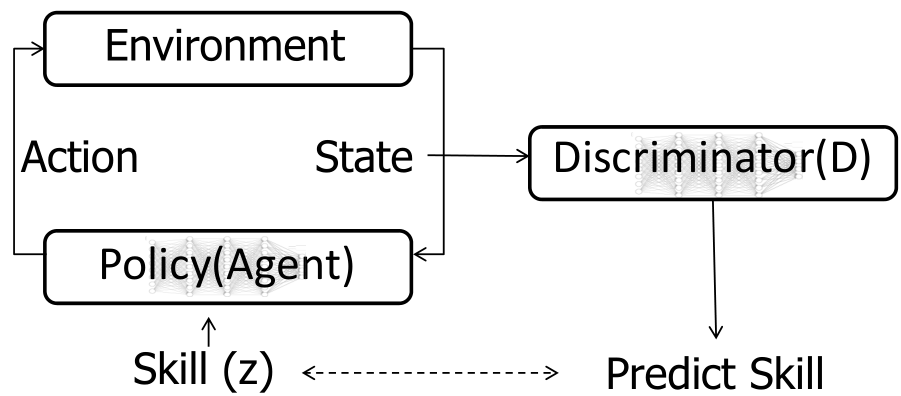
\includegraphics[width=.7\textwidth]{diayn.png}
	\caption{Diversity is All You Need. \cite{eysenbach2018diversity}.}
\end{figure}

\hlb{Connection to mutual information}
\begin{equation}
	\mathcal{I}(z,\textbf{s}) = \mathcal{H}(z) - \mathcal{H}(z|\textbf{s})
\end{equation}
\begin{itemize}
	\item $\mathcal{H}(z)$: maximized by using uniform prior $p(z)$
	\item $\mathcal{H}(z|\textbf{s})$: minimized by maximizing $r(\textbf{s}, z) = \log p(z|\textbf{s})$
\end{itemize}

\section{References}
\begin{itemize}
	\item \citeaus{schmidhuber1991possibility}. A possibility for implementing curiosity and boredom in model-building neural controllers.
	\item \citeaus{stadie2015incentivizing}. Incentivizing exploration in reinforcement learning with deep predictive models.
	\item \citeausm{osband2016deep}. Deep exploration via bootstrapped DQN.
	\item \citeausm{houthooft2016vime}. VIME: Variational Information Maximizing Exploration.
	\item \citeausm{bellemare2016unifying}. Unifying count-based exploration and intrinsic motivation.
	\item \citeausm{tang2017exploration}. \# exploration: A study of count-based exploration for deep reinforcement learning.
	\item \citeaus{fu2017ex2}. Ex2: Exploration with exemplar models for deep reinforcement learning.
\end{itemize}